\documentclass[titlepage,12pt]{article}
    \usepackage[utf8]{inputenc}
    \usepackage[margin=1in]{geometry}
    \usepackage{setspace}
    \usepackage{graphicx}
    \usepackage{titlepic}
    \usepackage[super]{nth}

    \graphicspath{ {images/} }

    \title{On Maurice Ravel's Work}
    \titlepic{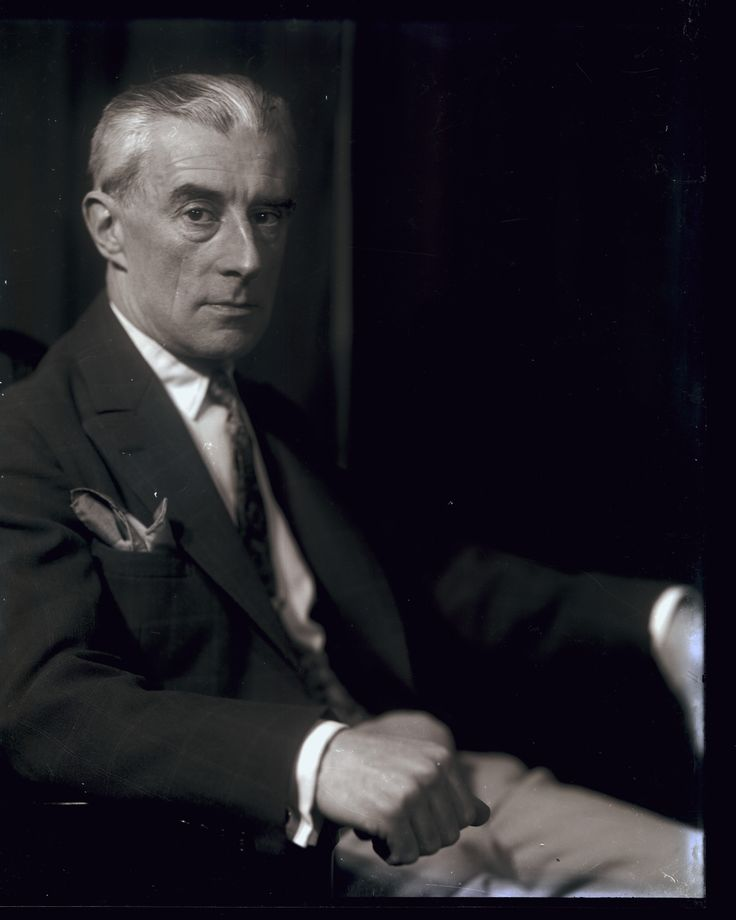
\includegraphics[width=200pt]{ravel.jpg}}
    \date{March 06, 2018}
    \author{Bernardo Meurer}
    \singlespacing
    \begin{document}
    \maketitle
    \newpage
    Maurice Ravel was a french composer and pianist from the \nth{20} century. Despite rejecting the categorization, it is wildly accepted that Ravel belonged to the impressionist movement, it becomes hard to argue against this taxonomization after listening to some of this great works, such as the ballet \textit{Daphnis et Chloè}, or even less known pieces such as his \textit{Piano Trio En La Mineur}. Overall, Ravel is one of the great minds of impressionism, together with Debussy who also rejected the title, and the quality of his work is beyond question.

    As a case study, we will look at his famed piano piece \textit{Pavane Pour Une Infante Defunte} (Literally ``Pavane For a Dead Child'', although usually translated as ``Pavane For a Dead Princess.'') The Pavane was initially composed in 1899, while Ravel was a student at the \textit{Conservatoire de Paris}, under the great French composer Gabriel Fauré, who unsurprisingly also composed a Pavane (in F-sharp minor) that received great acclaim. Later on, in 1910, Ravel published an orchestrated version of his Pavane, incorporating two flutes, oboe, two bassoons, two horns, harp, and strings. Despite the ``fuller'' sound of the orchestrated variation of Ravel's Pavane, by and large it fails to achieve the same level of emotion that the solo Piano performance can transmit.

    Before we go forward with out analysis, it's important to make explicit the marking characteristics of a Pavane proper. A Pavane is a slow dance that was common in the Renaissance era (\nth{16} Century) in European courts. The name ``Pavane'' probably originates from Italian ``Padovana'', which stands for ``Typical of Padua'', which is an Italian region. The name for Ravel's piece, ``Pavane for a dead Princess'', is due to his intent to write a Pavane that a small princess from the 16th century would have enjoyed dancing to in the palace halls, she is the dead princess, for now all of those who had enjoyed that pleasure are long gone.

    According to Ravel's biographer Benjamin Ivry, his Pavane was meant to be played \emph{extremely} slowly, much slower than any modern interpretation of it. This was gravely criticized at the time of his initial performances, with the some critics commenting that it was ``Unutterably slow.''

    Ravel's Pavane is composed in e-minor, which is extremely fitting of the general emotion that the piece is meant to transmit. As reference, it might be enough to listen to Chopin's Prelude in E-minor to appreciate how extremely depressant the key is. In the Pavane, this effect is still present, and very much so, the slow transitions of the piece, together with the large chords used cause a heavy impact on the listener. In particular, the distinction between the usage of high-pitched keys for the melodic work, and the polar opposite for the harmonic layer create an interesting contrast that adds to the general feeling impressed on the listener.

    Interestingly, what causes the Piano Solo version of the composition to be, arguably, the most emotionally impacting, is not the sound of the Piano, but the lack of it. The spacing, silence, in between chords and transitions allows for a greater interpretational depth from the listener, which deepens the involvement with the piece's overwhelming feeling of sadness, and perhaps a portion of nostalgia for the Dead Princess' time.

    Ravel's Pavane for a dead Princess, in e-minor, is a true impressionist masterpiece, and it shows, it's usage of color, harmony, and texture are a testament to the emotional capacity of the movement.
    \end{document}
